%%%%%%%%%%%%%%%%%%%%%%%%%%%%%%%%%%%%%%%%%
% Beamer Presentation
% LaTeX Template
% Version 1.0 (10/11/12)
%
% This template has been downloaded from:
% http://www.LaTeXTemplates.com
%
% License:
% CC BY-NC-SA 3.0 (http://creativecommons.org/licenses/by-nc-sa/3.0/)
%
%%%%%%%%%%%%%%%%%%%%%%%%%%%%%%%%%%%%%%%%%

%----------------------------------------------------------------------------------------
%	PACKAGES AND THEMES
%----------------------------------------------------------------------------------------

\documentclass{beamer}

\mode<presentation> {

% The Beamer class comes with a number of default slide themes
% which change the colors and layouts of slides. Below this is a list
% of all the themes, uncomment each in turn to see what they look like.

%\usetheme{default}
%\usetheme{AnnArbor}
%\usetheme{Antibes}
%\usetheme{Bergen}
%\usetheme{Berkeley}
%\usetheme{Berlin}
%\usetheme{Boadilla}
%\usetheme{CambridgeUS}
%\usetheme{Copenhagen}
%\usetheme{Darmstadt}
%\usetheme{Dresden}
%\usetheme{Frankfurt}
%\usetheme{Goettingen}
%\usetheme{Hannover}
%\usetheme{Ilmenau}
%\usetheme{JuanLesPins}
%\usetheme{Luebeck}
\usetheme{Madrid}
%\usetheme{Malmoe}
%\usetheme{Marburg}
%\usetheme{Montpellier}
%\usetheme{PaloAlto}
%\usetheme{Pittsburgh}
%\usetheme{Rochester}
%\usetheme{Singapore}
%\usetheme{Szeged}
%\usetheme{Warsaw}

% As well as themes, the Beamer class has a number of color themes
% for any slide theme. Uncomment each of these in turn to see how it
% changes the colors of your current slide theme.

%\usecolortheme{albatross}
\usecolortheme{beaver}
%\usecolortheme{beetle}
%\usecolortheme{crane}
%\usecolortheme{dolphin}
%\usecolortheme{dove}
%\usecolortheme{fly}
%\usecolortheme{lily}
%\usecolortheme{orchid}
%\usecolortheme{rose}
%\usecolortheme{seagull}
%\usecolortheme{seahorse}
%\usecolortheme{whale}
%\usecolortheme{wolverine}

%\setbeamertemplate{footline} % To remove the footer line in all slides uncomment this line
%\setbeamertemplate{footline}[page number] % To replace the footer line in all slides with a simple slide count uncomment this line

%\setbeamertemplate{navigation symbols}{} % To remove the navigation symbols from the bottom of all slides uncomment this line

\setbeamertemplate{frametitle}[default][center]
}

\usepackage{graphicx} % Allows including images
\usepackage{booktabs} % Allows the use of \toprule, \midrule and \bottomrule in tables
\usepackage{multimedia}
%\usepackage{movie15}
\usepackage{caption}
\usepackage{subcaption}
\usepackage{amsfonts}
\usepackage{epstopdf}
\usepackage{bigints}
\usepackage{amsmath}
\usepackage{hyperref}
\usepackage{verbatim}
\usepackage{mathrsfs}
\usepackage{color}
\usepackage[outline]{contour}
\usepackage{multirow}

\contourlength{1pt}

\newcommand\Bo{\mbox{\textit{Bo}}}  % Bond number
\newcommand\Rey{\mbox{\textit{Re}}}  % Reynolds number
\newcommand\Ri{\mbox{\textit{Ri}}}  % Richardson number

\def\Xint#1{\mathchoice
{\XXint\displaystyle\textstyle{#1}}%
{\XXint\textstyle\scriptstyle{#1}}%
{\XXint\scriptstyle\scriptscriptstyle{#1}}%
{\XXint\scriptscriptstyle\scriptscriptstyle{#1}}%
\!\int}
\def\XXint#1#2#3{{\setbox0=\hbox{$#1{#2#3}{\int}$}
\vcenter{\hbox{$#2#3$}}\kern-.5\wd0}}
\def\ddashint{\Xint=}
\def\dashint{\Xint-}

%----------------------------------------------------------------------------------------
%	TITLE PAGE
%----------------------------------------------------------------------------------------

\title[Modeling volcanic processes]{Magma transport processes} % The short title appears at the bottom of every slide, the full title is only on the title page

\author[Paul Jarvis]{Paul A. Jarvis} % Your name
\institute[UNIGE] % Your institution as it will appear on the bottom of every slide, may be shorthand to save space
{
\textit{paul.jarvis@unige.ch} % Your email address
}
\date{15th November 2019} % Date, can be changed to a custom date
\begin{columns}

  \begin{column}{0.33\paperwidth}
    $$
\includegraphics[width=0.3\paperwidth]{UNIGE_logo.jpg}$$
  \end{column}

  \begin{column}{0.33\paperwidth}
    $$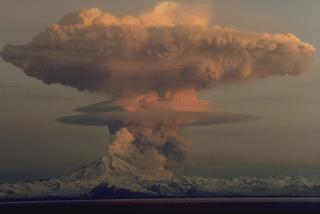
\includegraphics[width=0.3\paperwidth]{redoubt.jpg}$$
  \end{column}

  \begin{column}{0.33\paperwidth}
    $$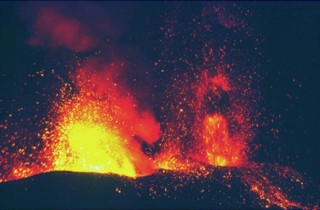
\includegraphics[width=0.3\paperwidth]{etna.jpg}$$
  \end{column}
  
\end{columns}
\vspace{-2cm}

\DeclareMathOperator\erf{erf}

\begin{document}

\begin{frame}
\titlepage % Print the title page as the first slide
\end{frame}

%\begin{frame}
%\frametitle{Overview} % Table of contents slide, comment this block out to remove it
%\tableofcontents % Throughout your presentation, if you choose to use \section{} and \subsection{} commands, these will automatically be printed on this slide as an overview of your presentation
%\end{frame}


%----------------------------------------------------------------------------------------
%	PRESENTATION SLIDES
%----------------------------------------------------------------------------------------

%------------------------------------------------
%\section{First Section} % Sections can be created in order to organize your presentation into discrete blocks, all sections and subsections are automatically printed in the table of contents as an overview of the talk
%------------------------------------------------

%\subsection{Subsection Example} % A subsection can be created just before a set of slides with a common theme to further break down your presentation into chunks

\begin{frame}
  \frametitle{Magmatic transport processes}

  \small Viscosity and density control how magma is transported within the Earth's crust \\

  Can consider transport of bulk magma, or fracionation of individual phases  \\

  \begin{columns}[t]

    \begin{column}{0.5\textwidth}

      \vspace{-1cm}
      
      $$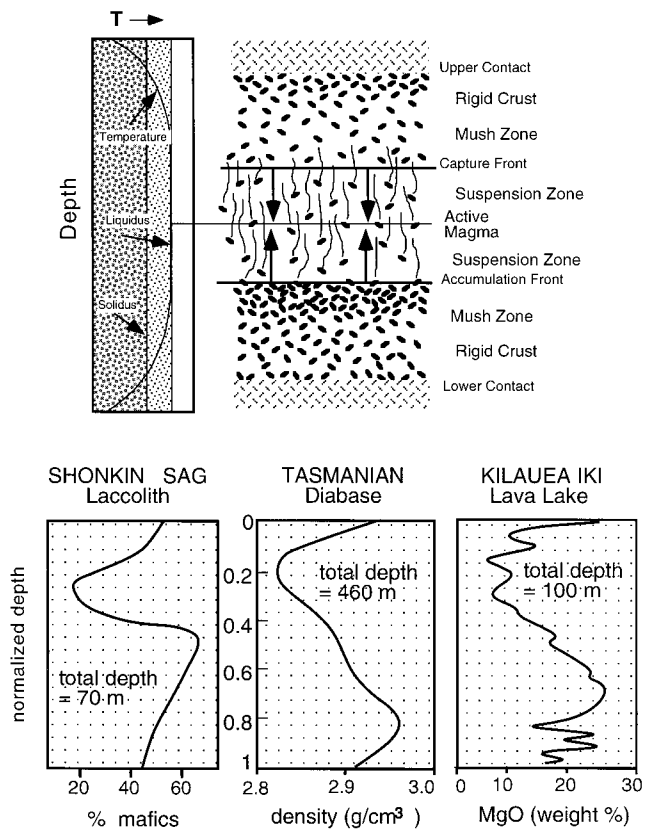
\includegraphics[width=0.9\textwidth]{crystals.png}$$

    \end{column}

    \begin{column}{0.5\textwidth}

      $$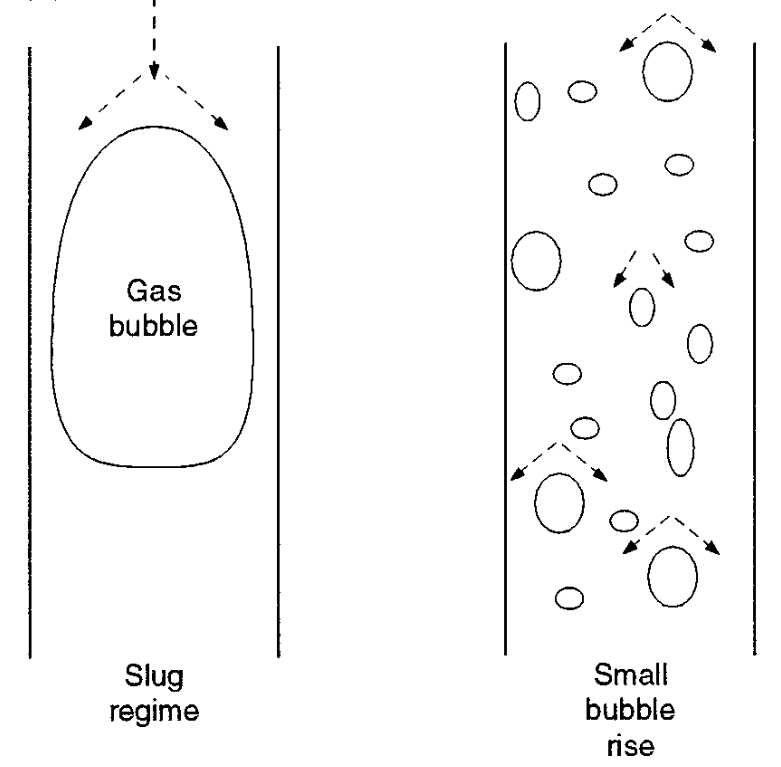
\includegraphics[width=0.95\textwidth]{bubbles.png}$$

    \end{column}
  \end{columns}
  
\end{frame}
%------------------------------------------------
\begin{frame}
  \frametitle{Crystal settling}

  Sills can contain cumulates - dense regions of crystals which have settled to the base of a chamber
  \begin{columns}[t]

    \begin{column}{0.5\textwidth}

      $$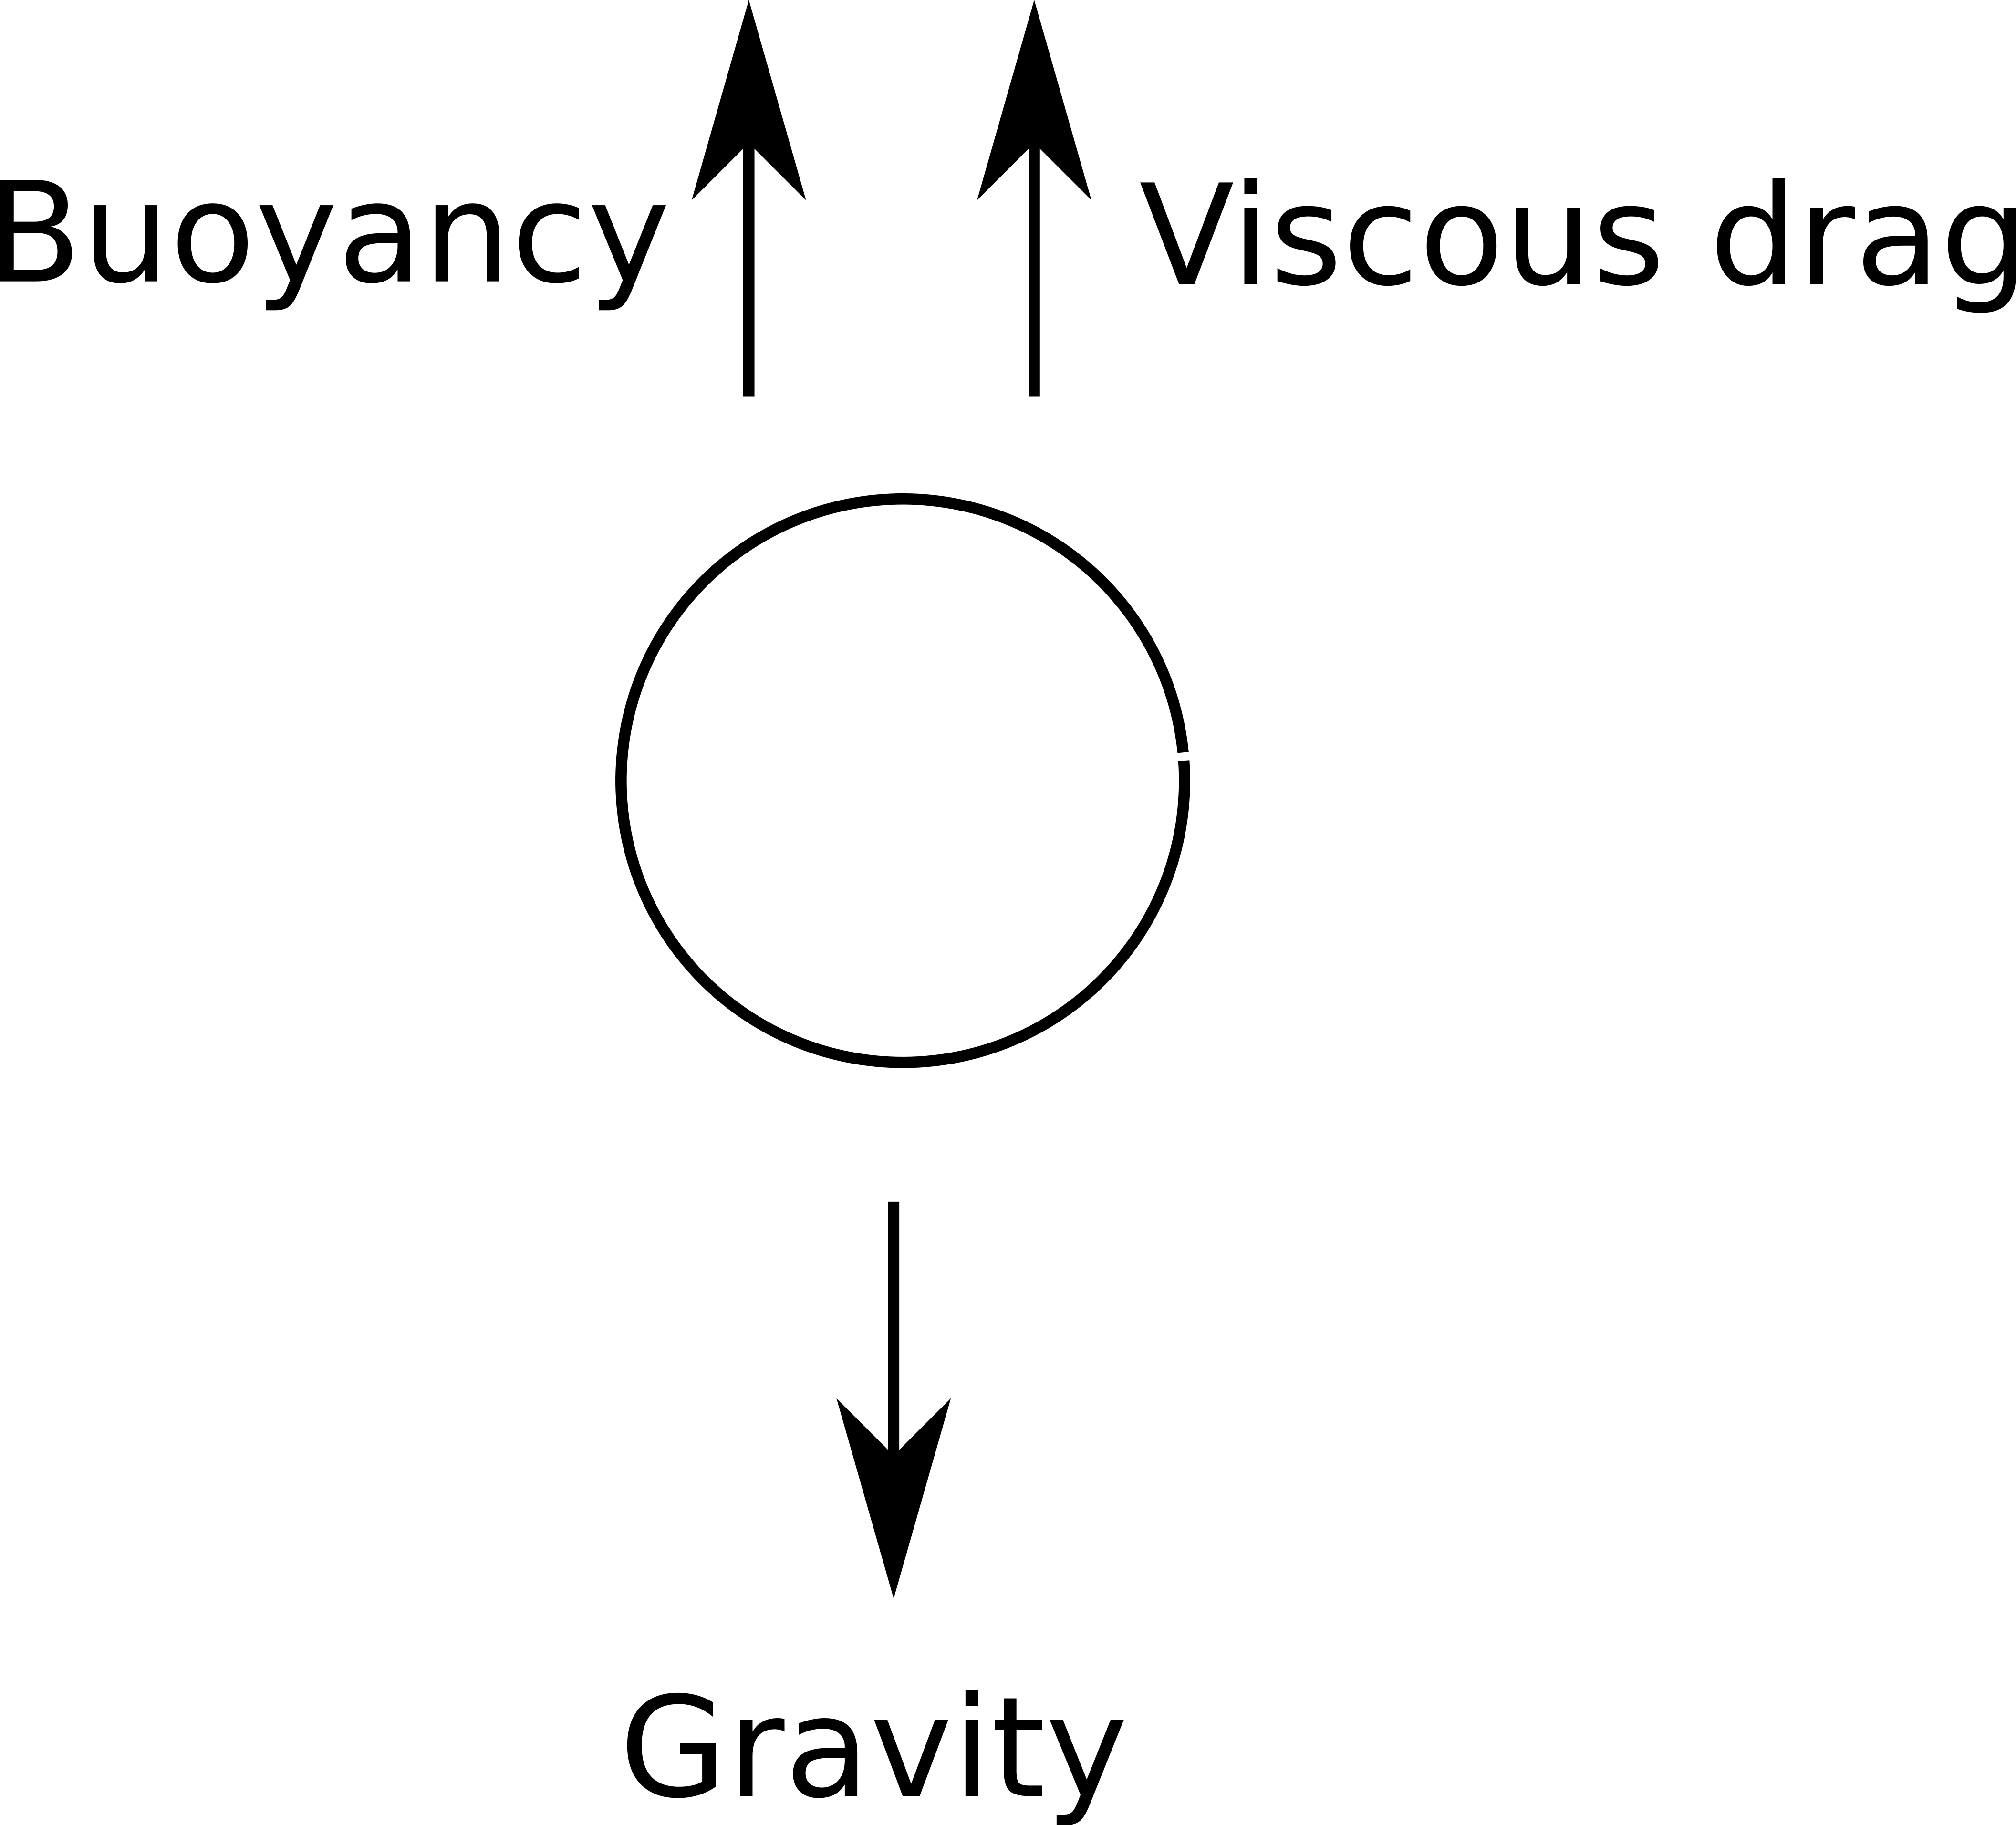
\includegraphics[width=0.9\textwidth]{stokes.png}$$

    \end{column}

    \begin{column}{0.5\textwidth}

      In viscous fluid, three forces act on sphere:

      \begin{itemize}
      \item Gravity $F_{\text{g}} = 4 \pi \rho_{\text{c}} r^{3} g / 3$ \\
      \item Buoyancy $F_{\text{b}} = 4 \pi \rho_{\text{m}} r^{3} g / 3$ \\
      \item Viscous drag $F_{\text{v}} = 6 \pi \eta_{\text{m}} r v_{\text{s}}$ \\
      \end{itemize}

      where $r$ = radius, $v_{\text{s}}$ = settling speed \\

      \vspace{0.5cm}
      
      In equilibrium $F_{\text{g}} = F_{\text{b}} + F_{\text{v}} \implies$ \\

      $$ v_{\text{s}} = \frac{2 (\rho_{\text{c}} - \rho_{\text{m}}) g r^{2}}{9 \eta_{\text{m}}} $$
    \end{column}
  \end{columns}
  
\end{frame}
%------------------------------------------------
\begin{frame}
  \frametitle{Bubble formation - volatile solubility}

  As magma rises, pressure falls and bubble solubility decreases \\

  \vspace{0.5cm}
  
  \textbf{Solubility} - Amount of substance that can be dissolved in a mixture \\

  \vspace{-0.5cm}
  
  \begin{columns}[t]

    \begin{column}{0.5\paperwidth}

      $$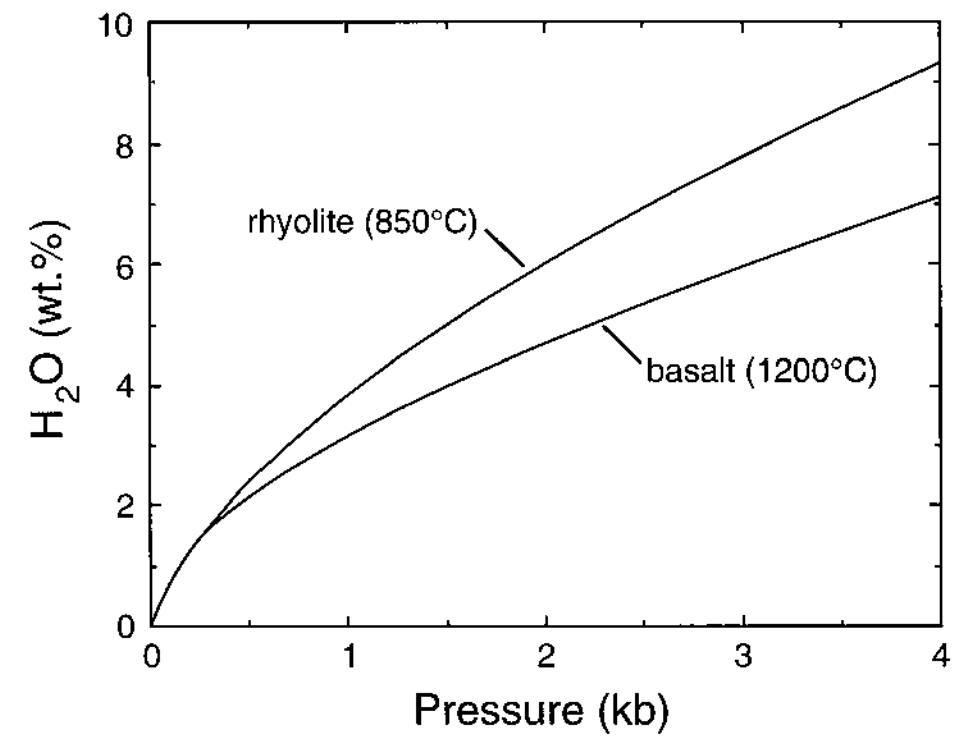
\includegraphics[width=0.95\textwidth]{P_H2O_phase.png}$$

    \end{column}

    \begin{column}{0.5\paperwidth}

      $$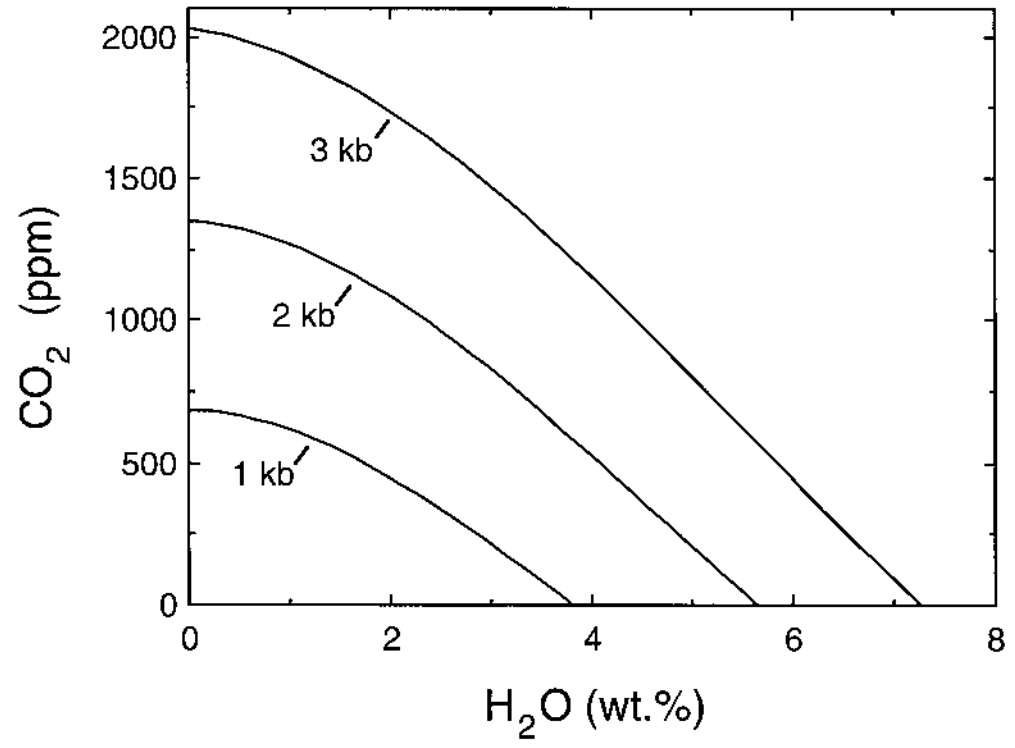
\includegraphics[width=0.95\textwidth]{CO2_H2O_P_phase.png}$$

    \end{column}
    
  \end{columns}

  If volatile concentrations exceed solubility, then magma is \textbf{supersaturated} \\
\end{frame}
%------------------------------------------------
\begin{frame}
  \frametitle{Bubble formation - Supersaturation}

  \textbf{Supersaturation} - Difference between actual pressure, and that at which concentration of dissolved volatiles would be in equilibrium

  \begin{columns}[t]

    \begin{column}{0.5\paperwidth}

      $$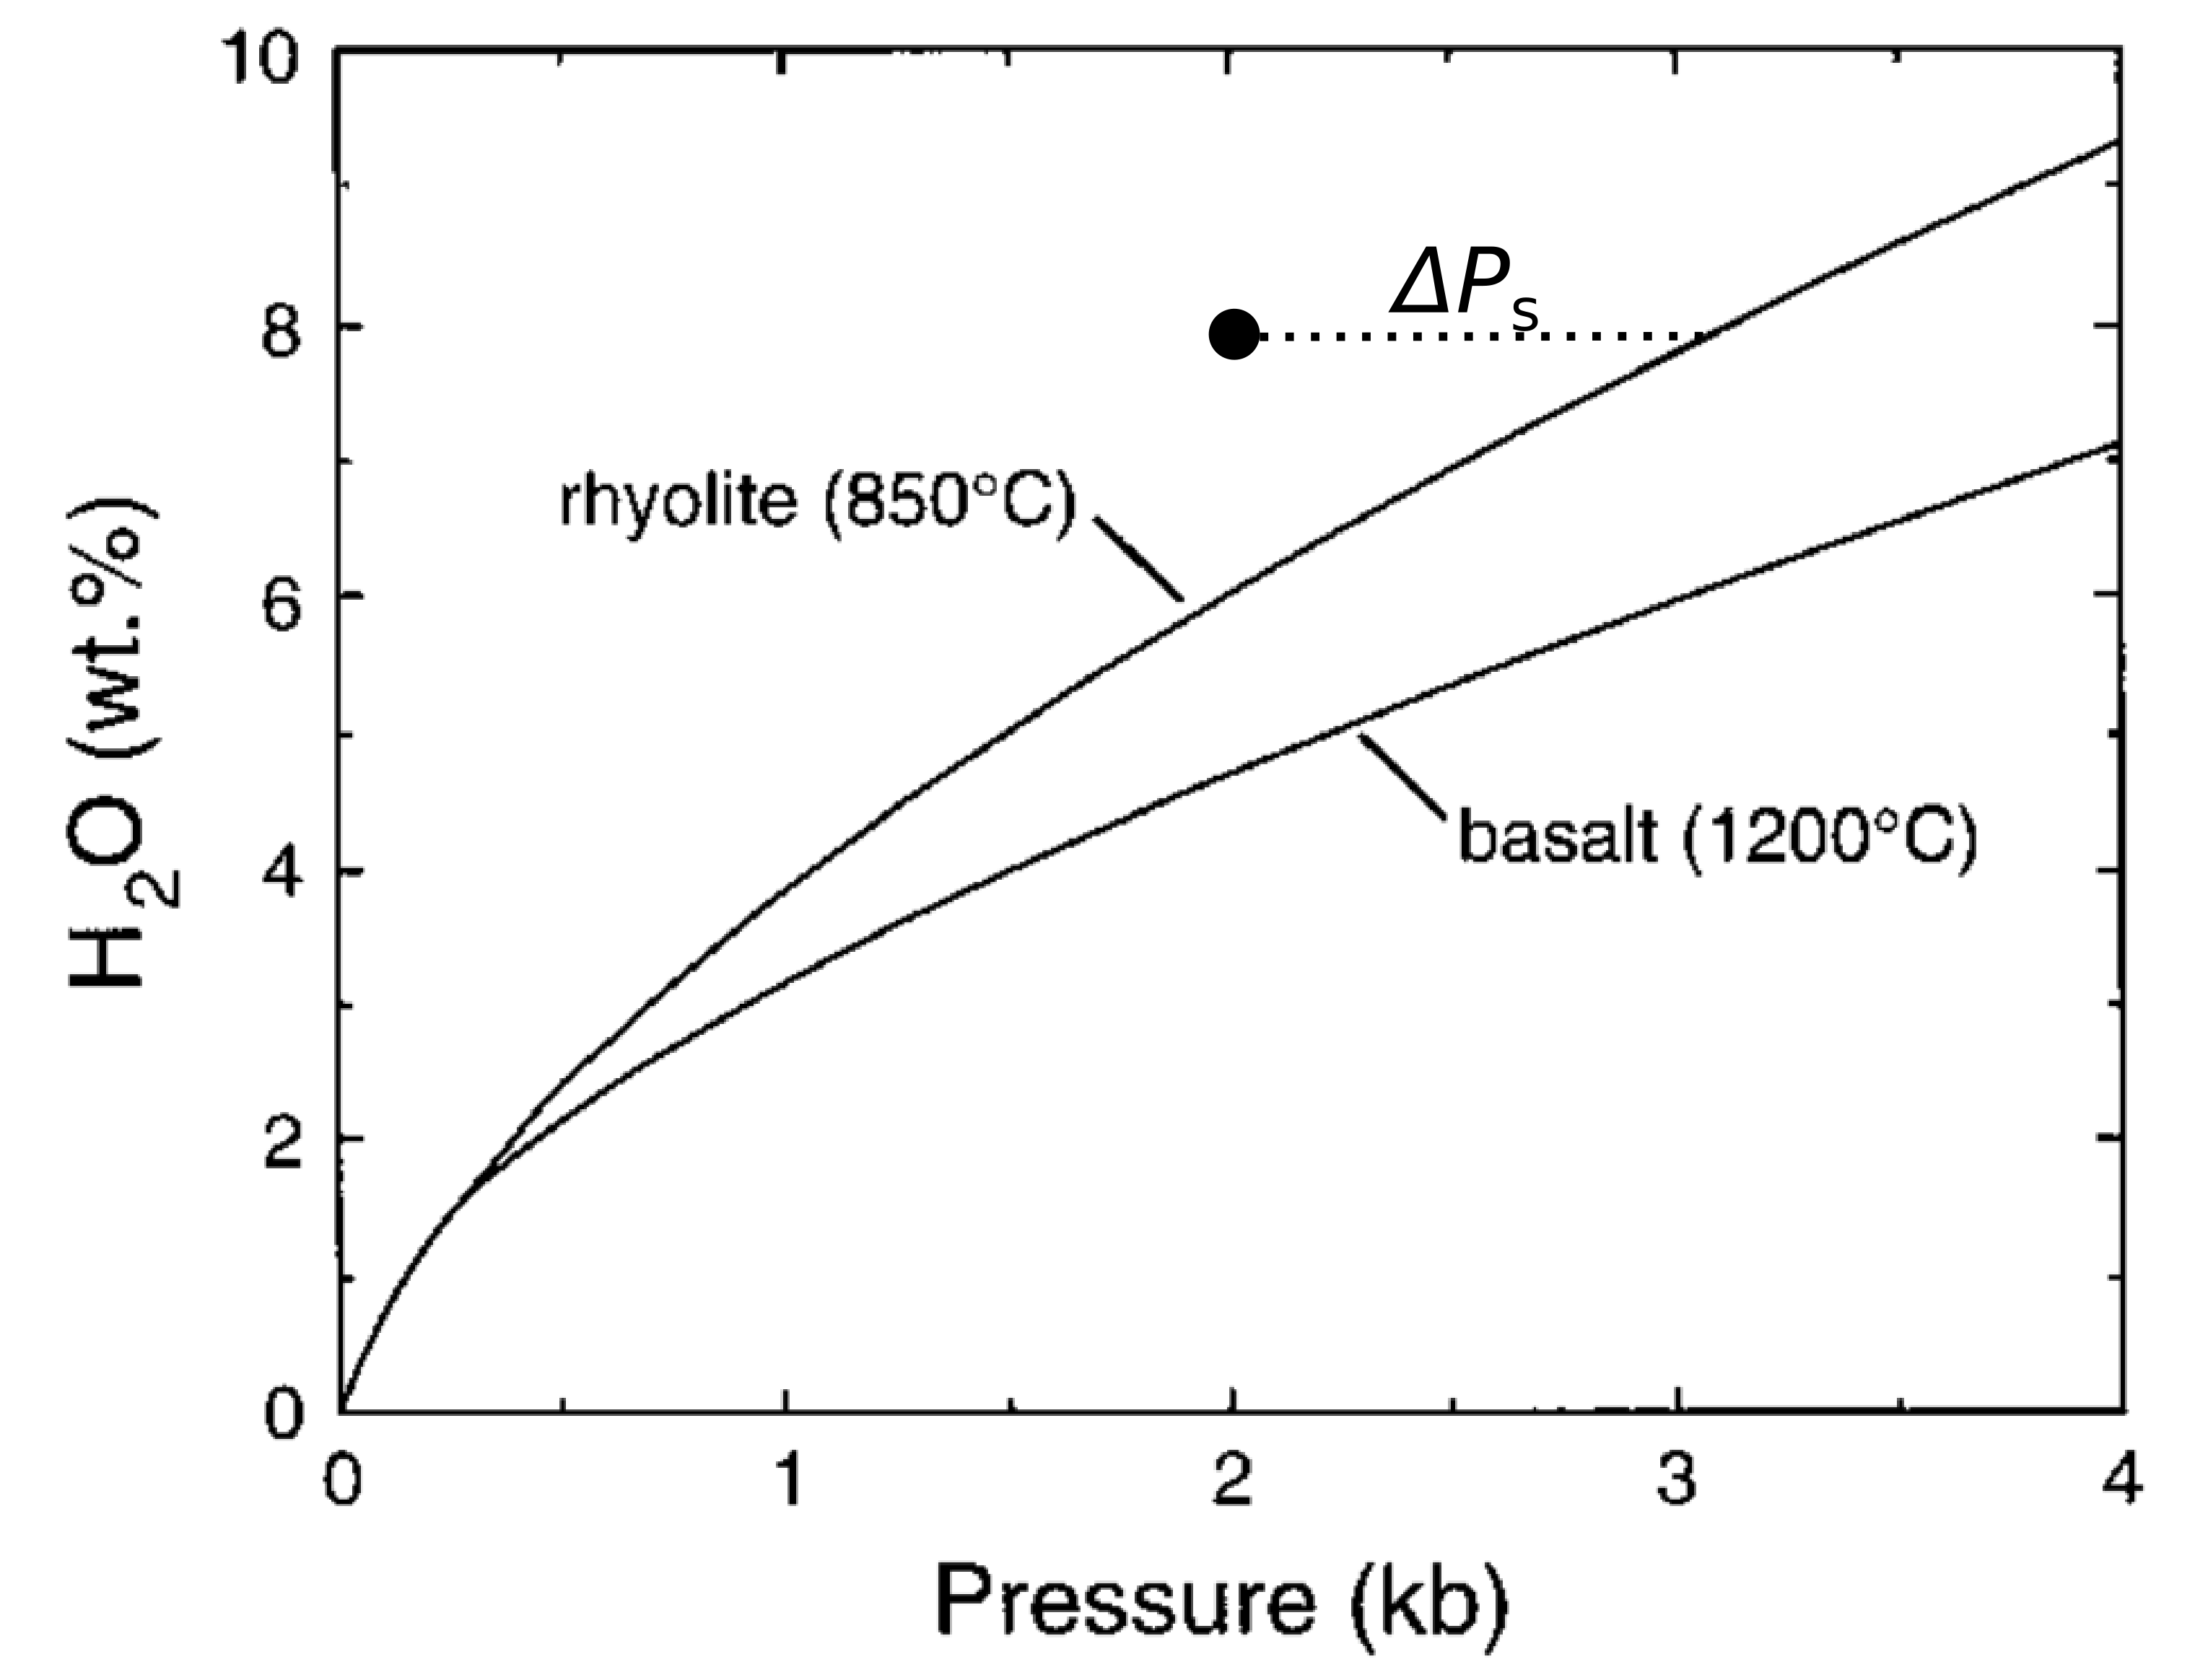
\includegraphics[width=0.95\textwidth]{supersat.png}$$

    \end{column}

    \begin{column}{0.5\paperwidth}

      \textbf{Nucleation} - Process by which bubbles initially form \\

      \vspace{0.5cm}

      Nucleation creates an interface between melt and volatile \\

      \vspace{0.5cm}

      \textbf{Interfacial tension} - Energy created to create an interface between two substances \\

      \vspace{0.5cm}

      Required amount of supersaturation corresponds to energy needed \\
    \end{column}
    
  \end{columns}
  
\end{frame}
%------------------------------------------------
\begin{frame}
  \frametitle{Bubble formation - Nucleation}

  Two types of nucleation:  
  \begin{columns}[t]

    \begin{column}{0.5\paperwidth}

      \centering \textbf{Homogeneous}

      \vspace{-0.5cm}
      
      $$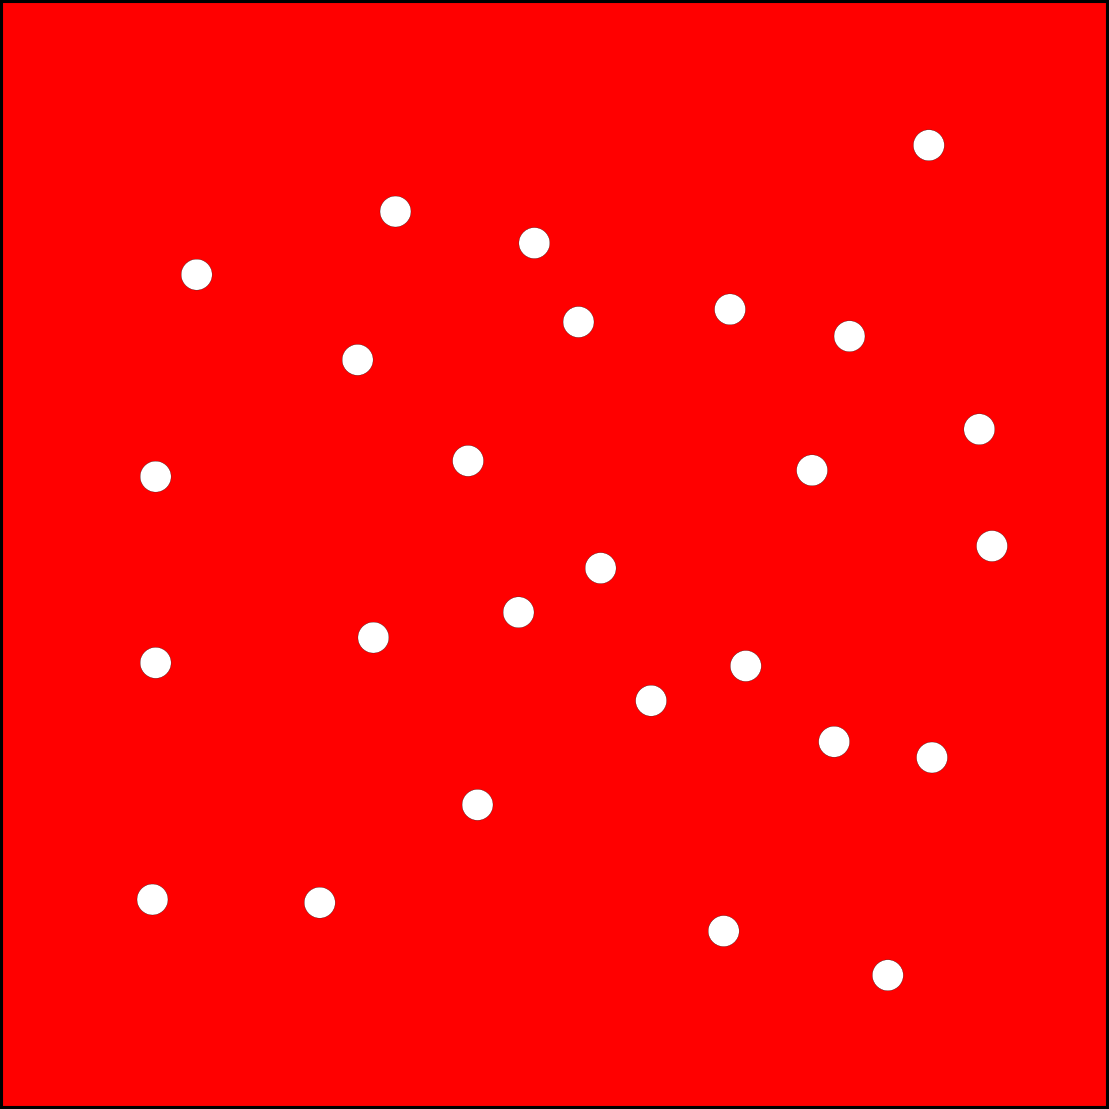
\includegraphics[width=0.95\textwidth]{homo_nuc.png}$$

    \end{column}

    \begin{column}{0.5\paperwidth}

      \centering \textbf{Heterogeneous}
      
      \vspace{-0.5cm}
      
      $$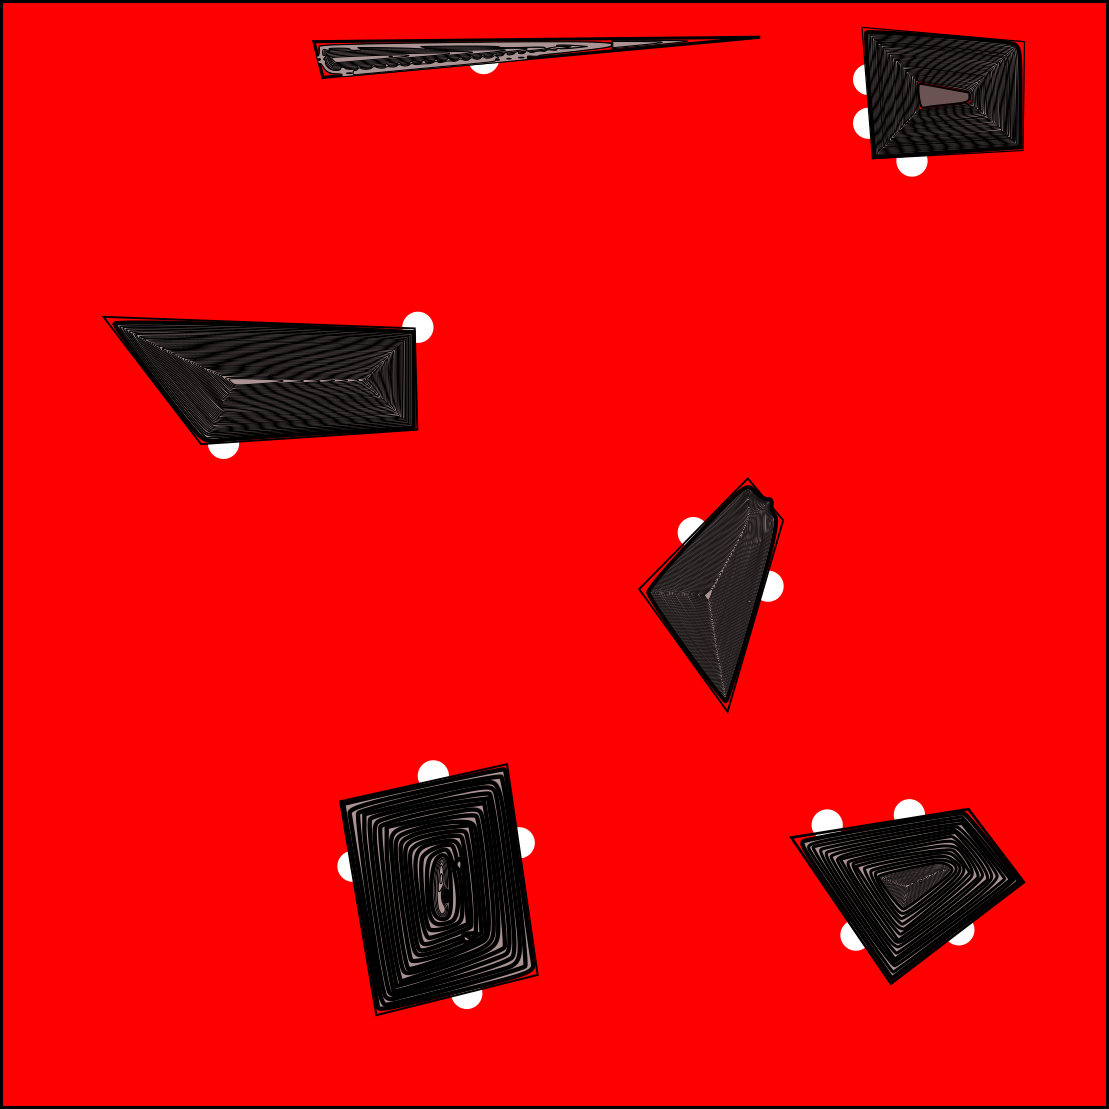
\includegraphics[width=0.95\textwidth]{hetero_nuc.png}$$
      
    \end{column}
    
  \end{columns}
  
\end{frame}
%------------------------------------------------
\begin{frame}
  \frametitle{Bubble formation - Homogenous nucleation}

  \begin{columns}[t]

    \begin{column}{0.5\paperwidth}

      \vspace{-0.5cm}
      
      $$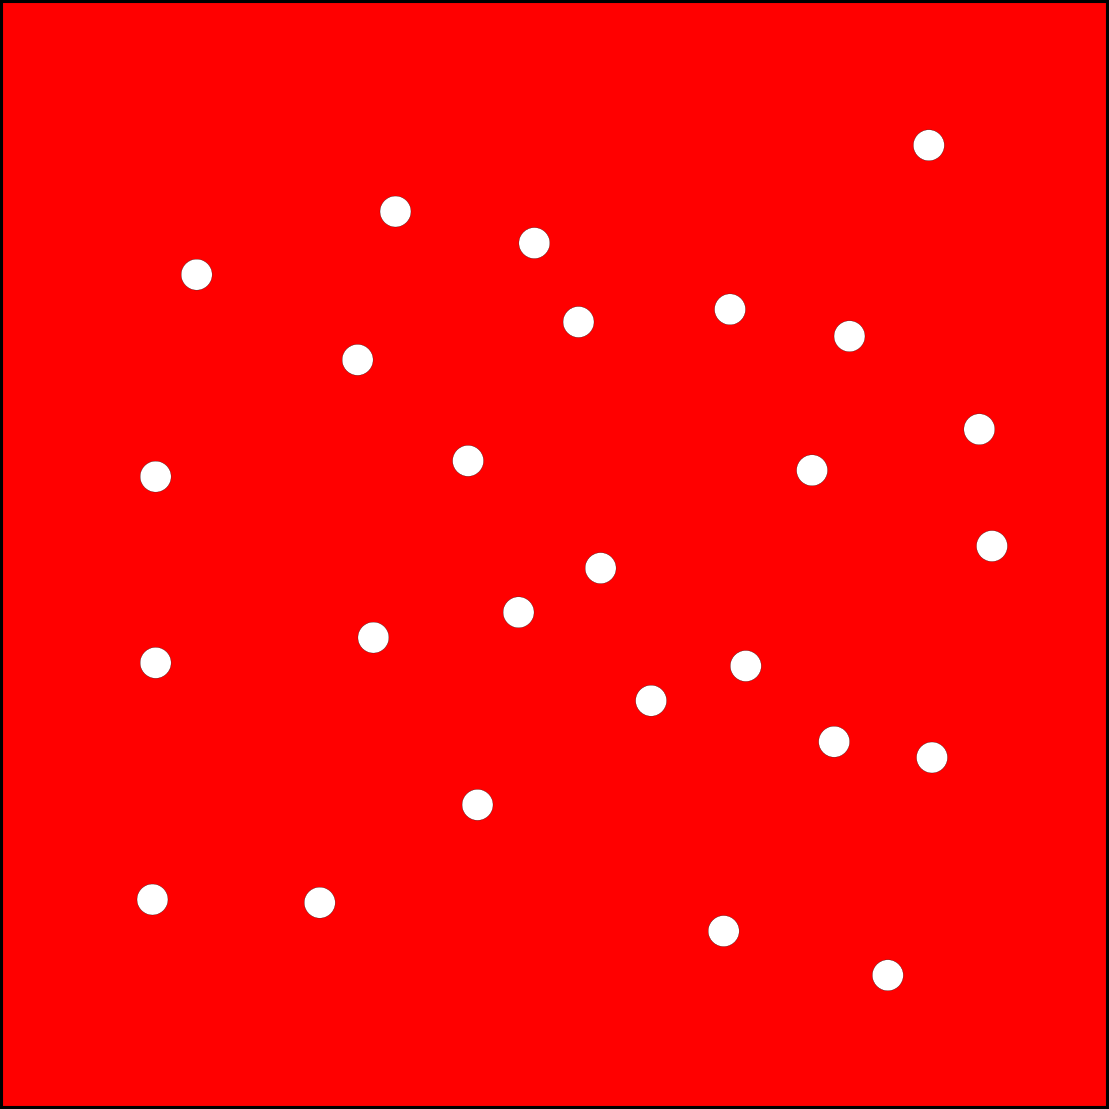
\includegraphics[width=0.95\textwidth]{homo_nuc.png}$$

    \end{column}

    \begin{column}{0.5\paperwidth}

      Occurs in the absence of crystals \\

      \vspace{2cm}

      Bubbles nucleate in the melt \\

      \vspace{2cm}

      Requires supersaturation of $\sim$ 10-100 MPa \\
    \end{column}
    
  \end{columns}
  
\end{frame}
%------------------------------------------------
\begin{frame}
  \frametitle{Bubble formation - Heterogeneous nucleation}

  \begin{columns}[t]

    \begin{column}{0.5\paperwidth}

      \vspace{-0.5cm}
      
      $$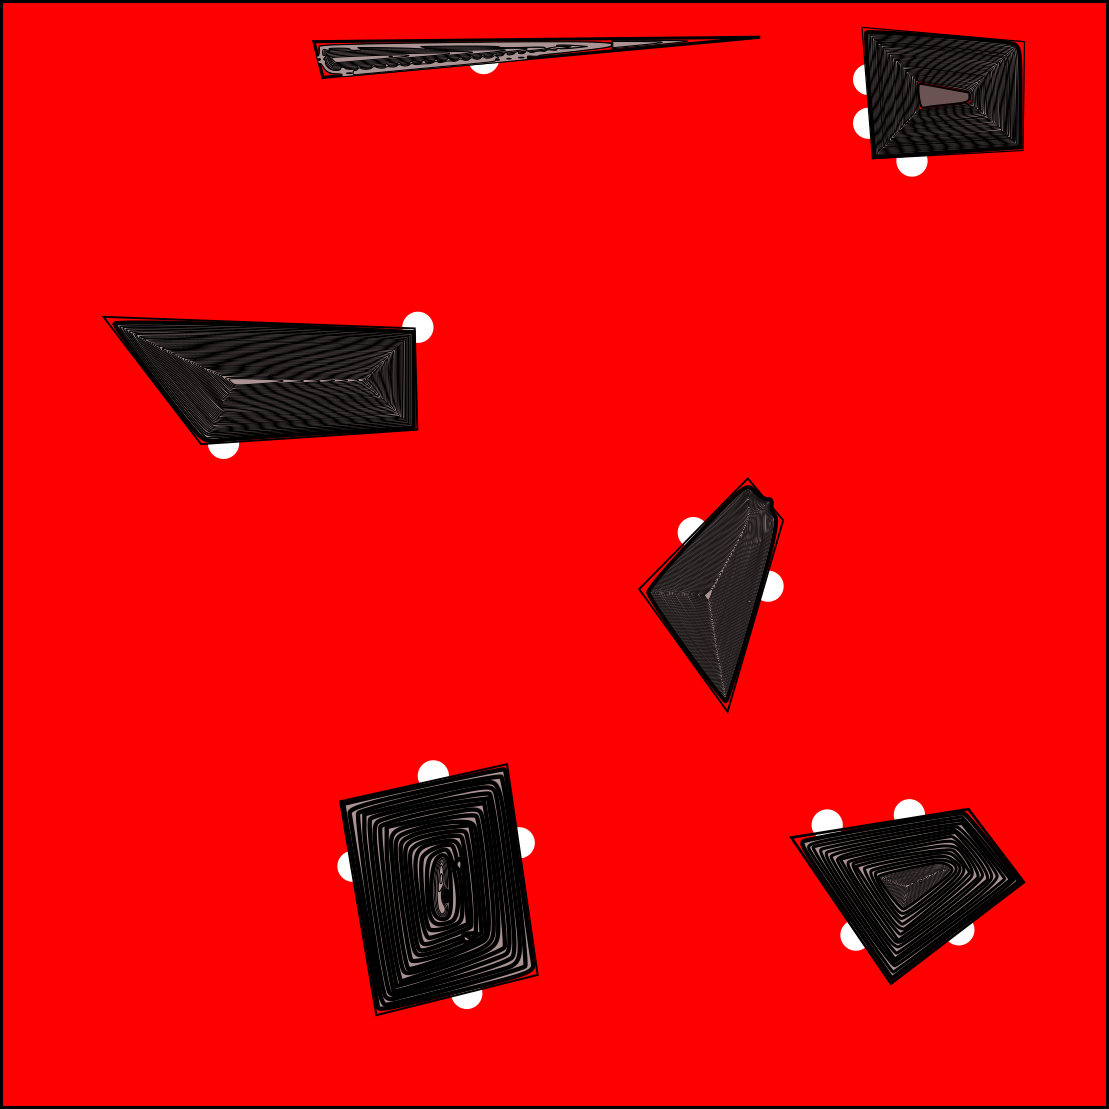
\includegraphics[width=0.95\textwidth]{hetero_nuc.png}$$

    \end{column}

    \begin{column}{0.5\paperwidth}

      Interfacial energy between vapour and crystal less than that between vapour and melt \\

      \vspace{1cm}

      Bubbles nucleate on crystals \\

      \vspace{1cm}

      Requires supersaturation of $\sim$ 1-10 MPa \\

      \vspace{1cm}

      $\implies$ in presence of crystals, nucleation will almost always be heterogeneous \\
    \end{column}
    
  \end{columns}
  
\end{frame}
%------------------------------------------------
\begin{frame}
  \frametitle{Bubble growth}

  \footnotesize As pressure decreases, bubbles grow due to expansion and increasing amount of exsolved gas \\

  3 regimes of bubble growth:

  \begin{itemize}
  \item Viscosity-limited growth
    \begin{itemize}
      \footnotesize 
      \item Melt viscosity is sufficiently high to slow down bubble expansion \\
      \item Leads to large supersaturation and build up of over-pressure in bubbles (mechanical disequilibrium) \\
      \item Significant for $\eta_{\text{m}} \geq 10^{9}$ Pa s (silicic melts at shallow depths and low $X_{\text{H}_{2}\text{O}}$ \\
    \end{itemize}

  \item Diffusion-limited growth
    \begin{itemize}
    \footnotesize
    \item Melt diffusivity is too low for oversaturated volatiles to diffuse to pre-existing bubbles (chemical disequilibrium) \\
    \item Leads to nucleation at the expense of growth \\
    \item Results in many small bubbles \\
    \end{itemize}

  \item Solubility-limited growth
    \begin{itemize}
    \footnotesize
    \item Diffusivity high, and viscosity low, enough to allow mechanical and chemical equilibrium \\
    \item Bubbles can grow unhindered \\
    \item Favoured for low melt viscosity (hot, mafic) and low ascent rates \\
    \end{itemize}
  \end{itemize}
\end{frame}
%------------------------------------------------
\begin{frame}
  \frametitle{Bubble rise speed}

  Bubble rise speed can be estimated by assuming spherical shape and using Stokes law

  $$ v_{\text{b}} = \frac{(\rho_{\text{m}} - \rho_{\text{b}}) g d^{2}}{18 \eta_{\text{m}}}$$

  \begin{columns}[t]

    \begin{column}{0.5\paperwidth}

      Depends on:
      \begin{itemize}
      \item $\rho_{\text{m}}$ = Melt density \\
      \item $\rho_{\text{b}}$ = Bubble density \\
      \item $d$ = Bubble diameter \\
      \item $\eta_{\text{m}}$ = Melt viscosity \\
      \end{itemize}

    \end{column}

    \begin{column}{0.5\paperwidth}

      Other factors:
      \begin{itemize}
      \item Bubble shape \\
      \item Bubble concentration $\phi_{\text{b}}$ \\
      \item Crystal fraction $\phi_{\text{c}}$ \\
      \end{itemize}

    \end{column}

  \end{columns}
  
\end{frame}
%------------------------------------------------
\begin{frame}
  \frametitle{Bubble flow regimes}

  \centering $v_{\text{b}}$ = Bubble speed, $v_{\text{m}}$ = Melt speed \\
  \begin{columns}[t]

    \begin{column}{0.5\paperwidth}

      \vspace{-1cm}
      
      $$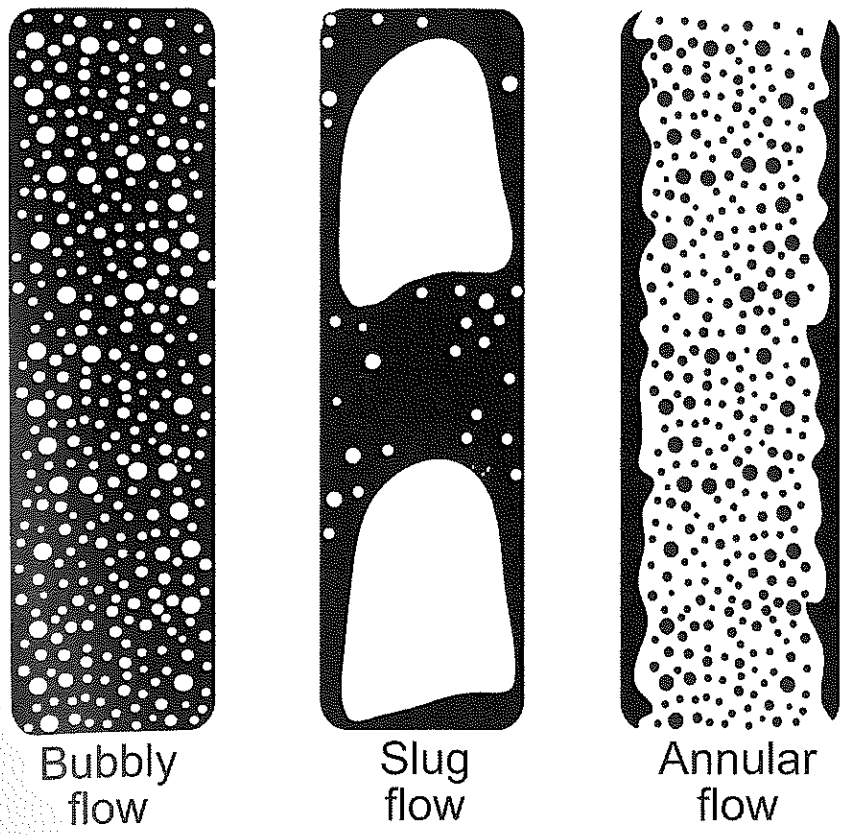
\includegraphics[width=0.95\textwidth]{gas_flow.png}$$
      
    \end{column}

    \begin{column}{0.5\paperwidth}

      If $v_{\text{b}} \ll v_{\text{m}} \implies$ \textbf{dispersed flow}:

      \begin{itemize}
      \item \textbf{Bubbly flow}
      \item Bubbles dispersed \\
      \item Move as passive tracers \\
      \end{itemize}

      If $v_{\text{b}} \gtrsim v_{\text{m}} \implies$ \textbf{separated flow}

      \begin{itemize}
        \item $ 1 \lesssim v_{\text{b}} / v_{\text{m}} \lesssim 10 \implies$ \textbf{slug flow} \\
        \item $ v_{\text{b}} / v_{\text{m}} \gtrsim 10 \implies$ \textbf{annular flow}
      \end{itemize}
    \end{column}
  \end{columns}

  Flow regimes are observed for gas flow in a vertical pipe \\

  Application to volcanic conduits remains debatable \\
\end{frame}
%------------------------------------------------
\begin{frame}
  \frametitle{Conduit flow}

  \begin{columns}[t]

    \begin{column}{0.48\paperwidth}

      $$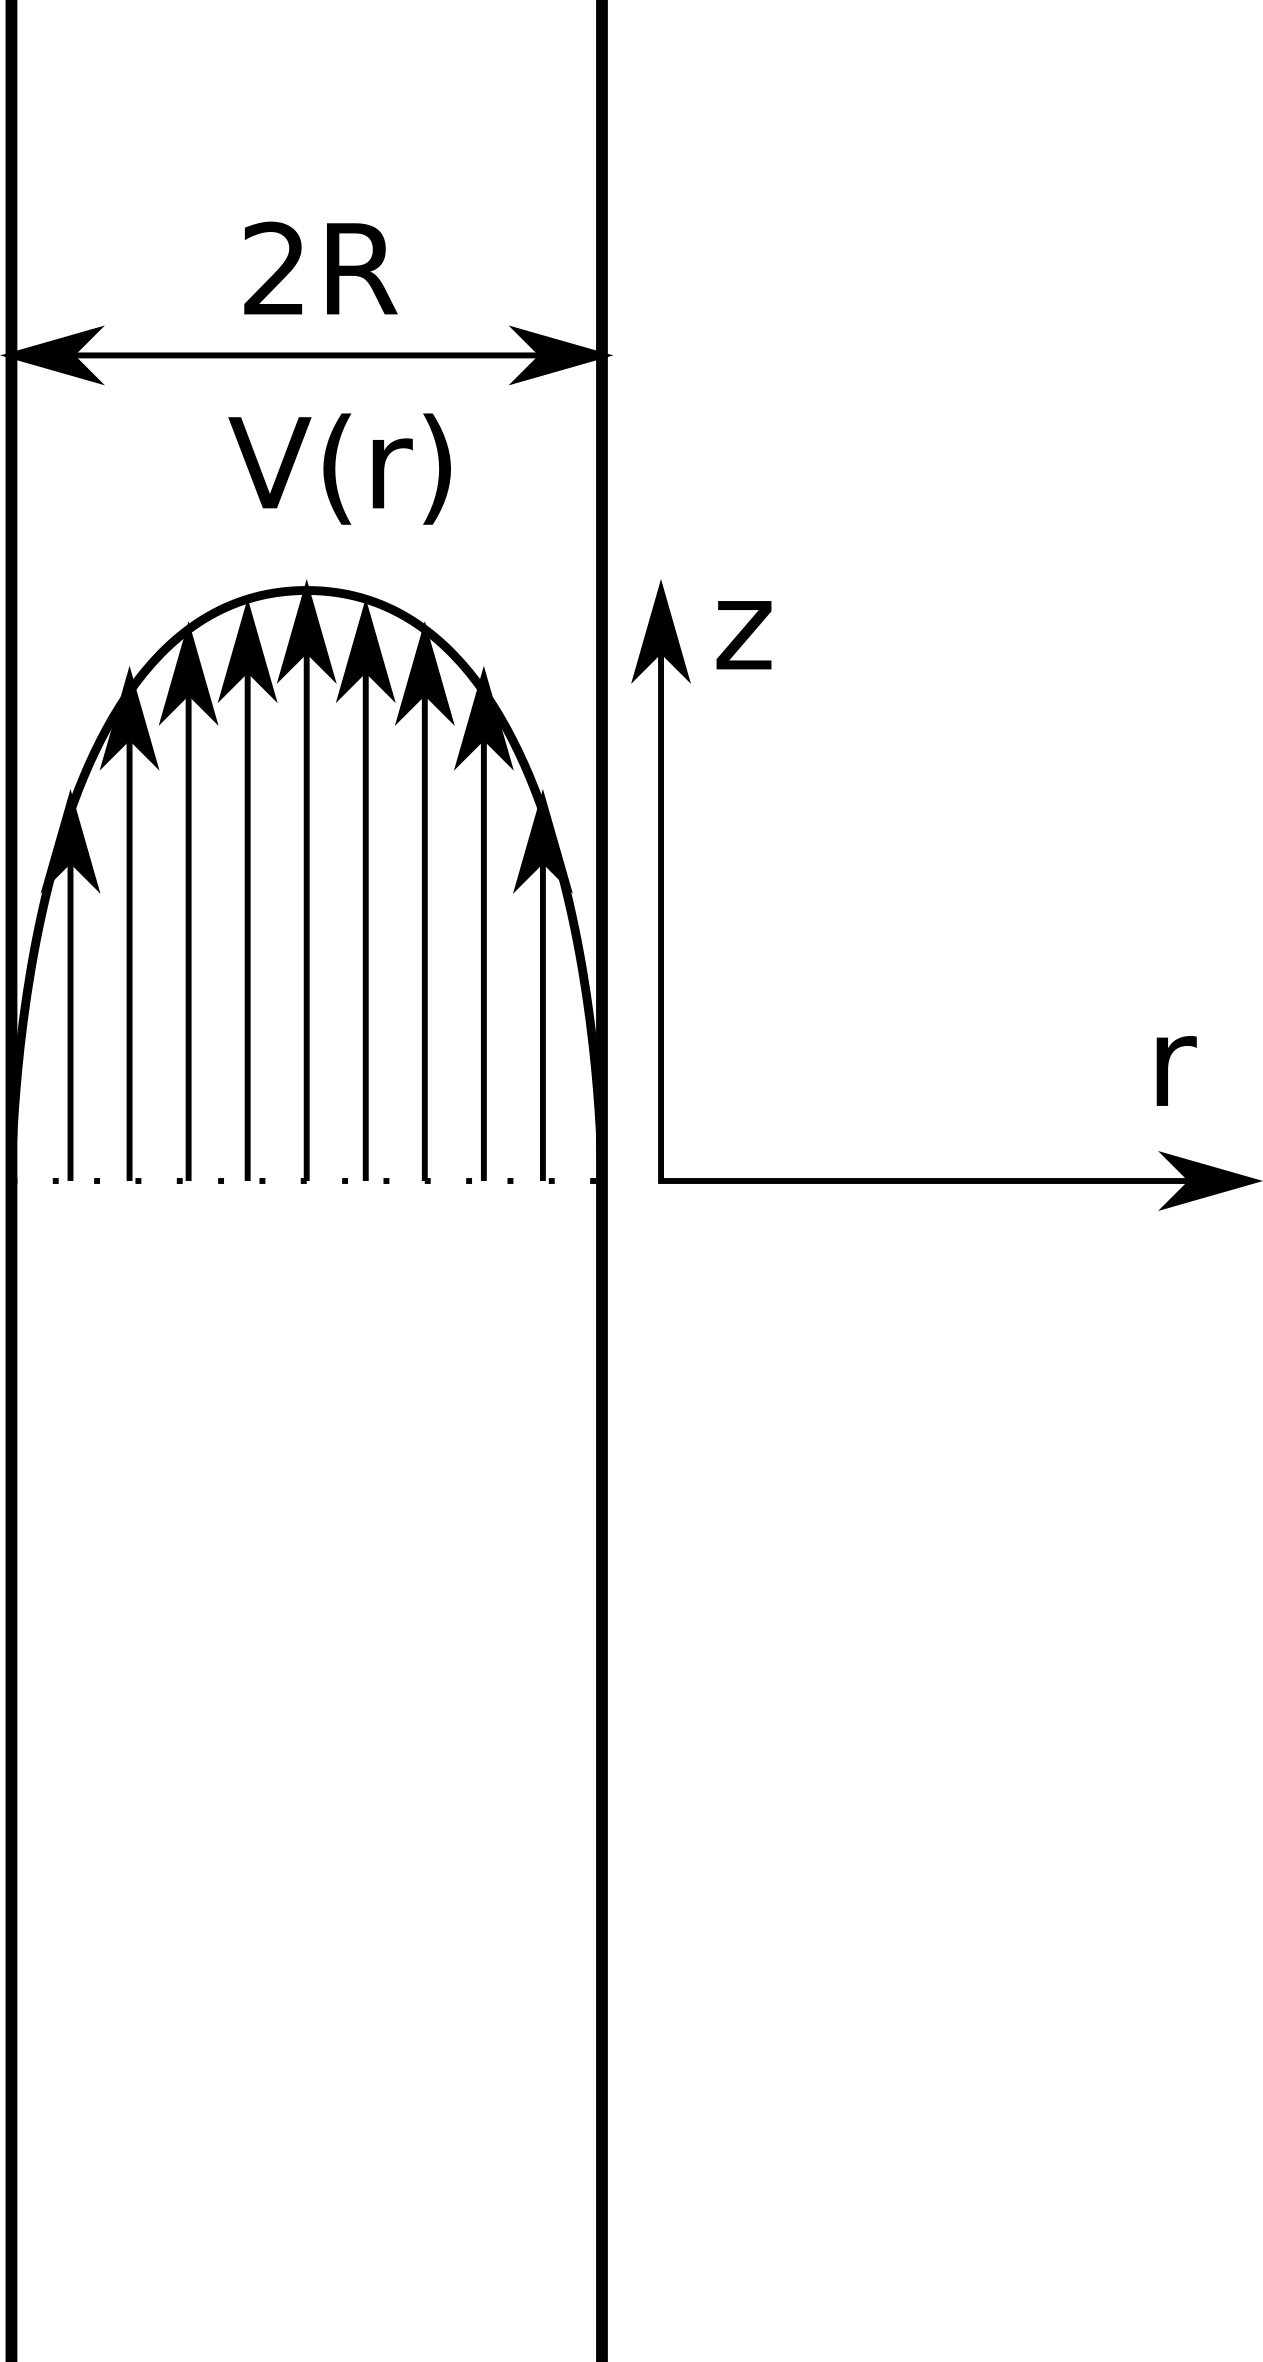
\includegraphics[width=0.5\textwidth]{conduit.png}$$
      
    \end{column}

    \begin{column}{0.5\paperwidth}

      Flow driven by pressure gradient $\mathrm{d} P / \mathrm{d} z$ \\

      Velocity profile given by

      $$ \frac{\mathrm{d} V}{\mathrm{d} r} = \frac{r}{2 \eta} \frac{\mathrm{d} P}{\mathrm{d} z} $$

      Friction with conduit walls means flow is fastest in centre \\

      Model is valid if flow is NOT separated \\
    \end{column}
  \end{columns}
\end{frame}
%------------------------------------------------
\begin{frame}
  \frametitle{Fragmentation}

  \textbf{Fragmentation} - During explosive eruptions, magma fragements to form \textbf{pyroclasts} - ash, lapilli, bombs \\

  \begin{itemize}
  \item Style of fragmentation depends on magma rheology \\
  \item In turn depends on $\phi_{\text{c}}, \phi_{\text{b}}, \eta_{\text{m}}, \dot{\epsilon}$
  \item Controls style of eruption \\
  \end{itemize}

  \begin{columns}[t]

    \begin{column}{0.37\paperwidth}

      $$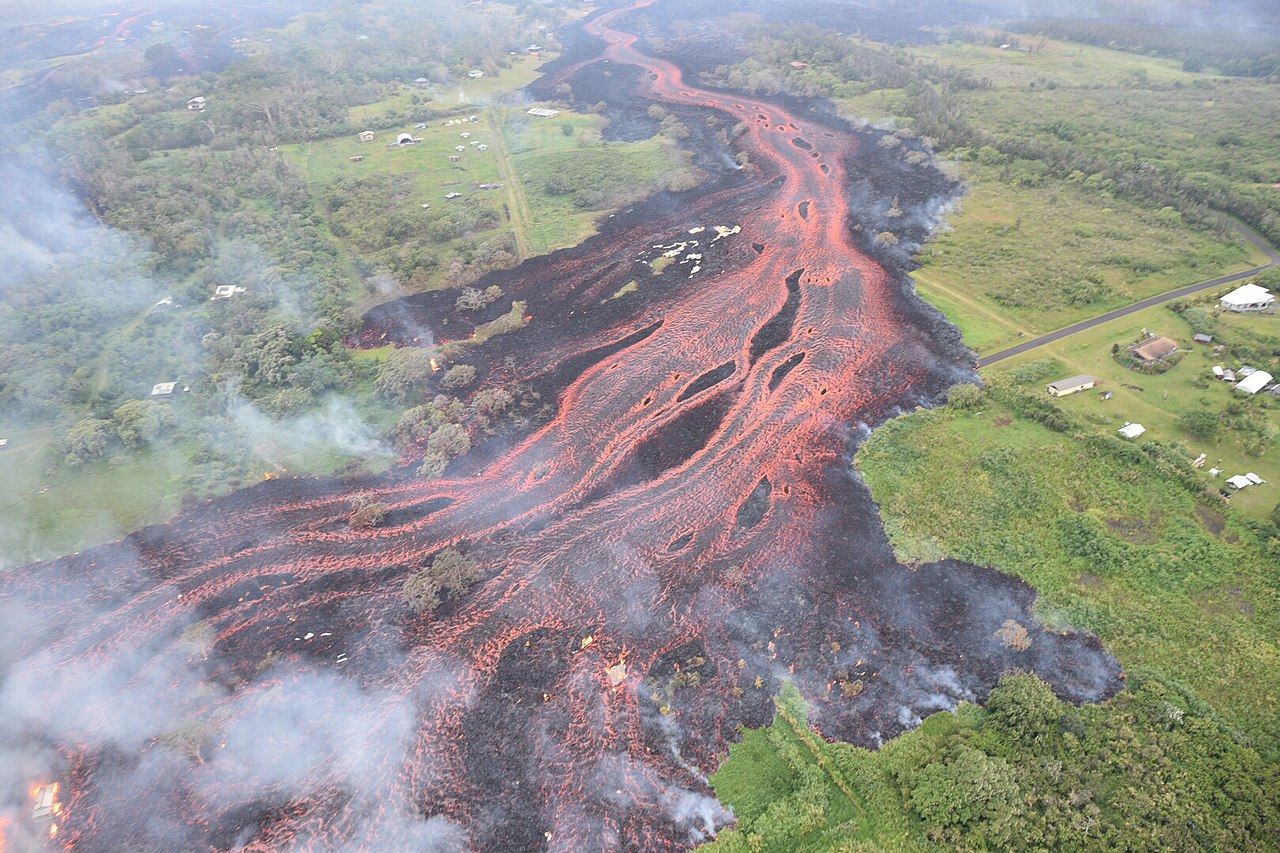
\includegraphics[width=\textwidth]{flow.jpg}$$

    \end{column}

    \begin{column}{0.25\paperwidth}

      $$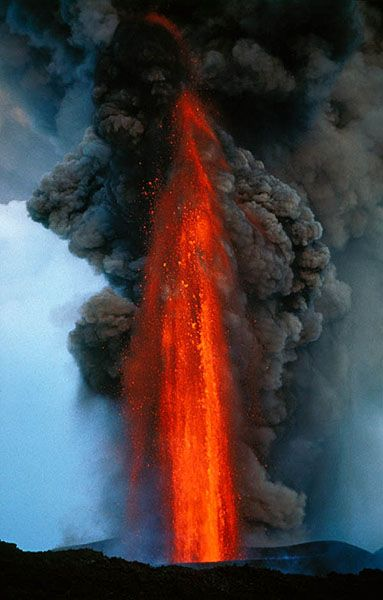
\includegraphics[width=0.9\textwidth]{fountain.jpg}$$

    \end{column}

    \begin{column}{0.37\paperwidth}

      $$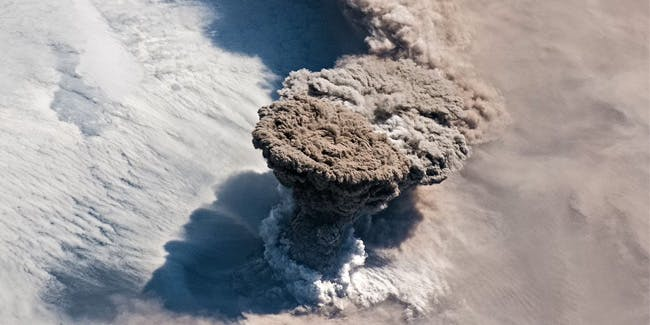
\includegraphics[width=\textwidth]{plume.jpeg}$$
      
    \end{column}
  \end{columns}
\end{frame}
%------------------------------------------------
\begin{frame}
  \frametitle{Magma mixing and mingling}

  \textbf{Magma mixing and mingling} - Magmas of different compositions juxtapose and interact \\

  \begin{itemize}
  \item Viscosity and density contrasts between magmas inhibit mixing \\
  \item Heat transfer fromm hot to cold magma associated with rheological changes \\
  \item Style of mixing changes with time \\
  \end{itemize}

  \vspace{-1cm}
  
  \begin{columns}[t]

    \begin{column}{0.66\paperwidth}

      $$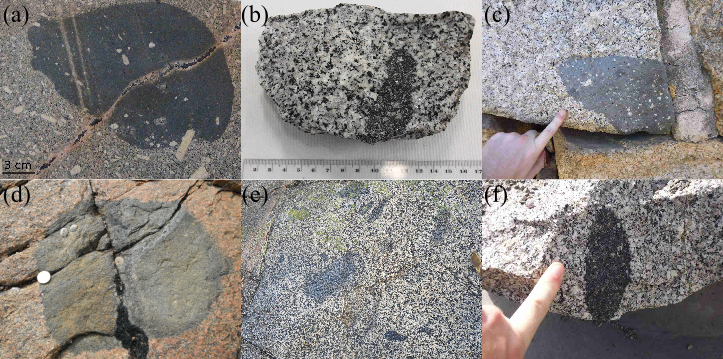
\includegraphics[width=0.9\textwidth]{figure1.png}$$

    \end{column}

    \begin{column}{0.33\paperwidth}

      $$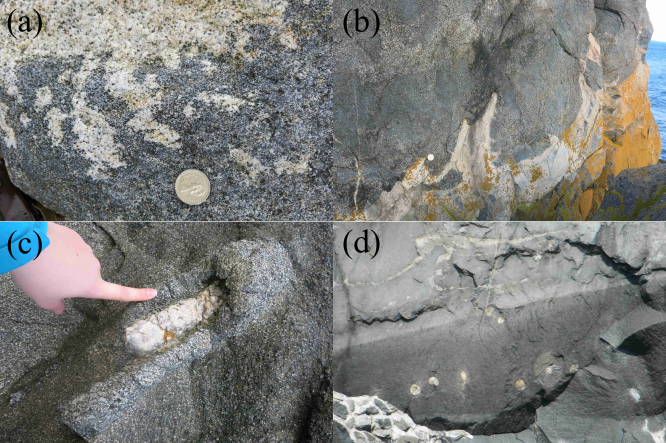
\includegraphics[width=0.9\textwidth]{figure2.png}$$

    \end{column}

  \end{columns}
  
\end{frame}
%------------------------------------------------


\end{document}
